\section{Protección de contenido con derechos de autor en Miracast}

Con el claro objetivo de ser un cable HDMI pero sin el cable, Miracast provee una interfaz con la cual permite abstraerse completamente sobre los codecs usados por los distintos dispositivos, pero esto plantea la duda acerca de cómo se gestionan los contenidos con copiright. Para ello Miracast provee su propio DRM (Digital Rights Management), el cual emula el sistema usado por los dispositivos HDMI, para dicho propósito usa HDCP, especificación propietaria y desarrollada por Intel con dicho cometido.

Para ello y por requerimiendo de DHCP, si el dispositivo emisor comunica que se van a enviar contenidos protegidos el receptor debe tener implementado su propio gestor de DHCP, que al haber sido licenciado garantiza que el dispositivo receptor debe de frustar los intentos de copia, para así evitar que el contenido sea distribuido libremente o copiado sin previa autorización.

Así si el dispositivo receptor no cumple con esta especificación solo recibe una señal peor de la real, con esto se busca evitar precisamente esa violación de los contenidos con derechos de autor.

Miracast requiere dependiendo de su versión del uso de DHCP en la version 2.1 o 2.2 de dicha especificación, cuyo funcionamiento en dispositivos que esten retransmitiendo por medio de Miracast es el siguiente:

\subsection{Gestión de DHCP en el servidor de contenidos Miracast}

El servidor, de ahora en adelante el dispositivo que emite contenido mediante Miracast, comprueba periódicamente si ha de enviar contenido protegido, si esta comprobación es afirmativa se envian una serie de bits cifrados durante la transmisión que solo si el receptor es capaz de decodificar (lo que indica que cumple con la especificación de DHCP) serán gestionables y además se enviará un feedback al emisor para confirmar la recepcion y correcta gestión de dichos datos. Como se muestra en la figura siguiente, ésto se lleva a cabo en la capa de TCP de transmisión de datos, mediante una conexión con la implementacion de DHCP del dispositivo emisor:

\begin{figure}[ht]
  \begin{centering}
    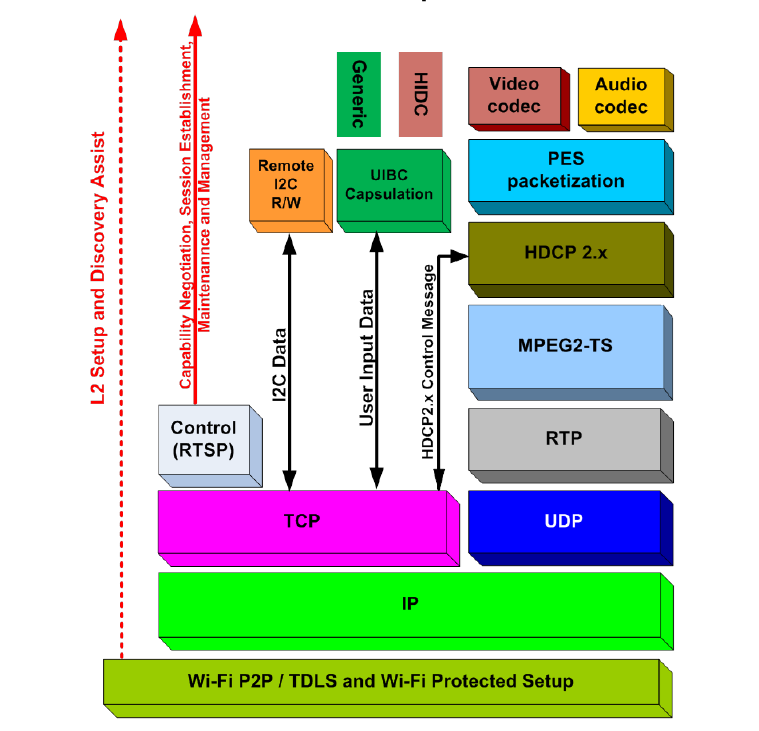
\includegraphics[width=1.0\textwidth]{./Imagenes/HDCP_miracast_layers.png}
    \caption{Ilustración acerca de dónde se ubica HDCP en el protocolo de conexión Miracast}
  \end{centering}
\end{figure}

El receptor simplemente hace la comprobación y gestiona los datos devolviendo un feedback al emisor, por lo que todo el coste de la gestión de DRM recae sobre él.
